\chapter{Analyse et Conception}

L'analyse et la conception constituent les phases cruciales dans le développement de tout système d'information. Cette étape permet de transformer les besoins exprimés par les utilisateurs en spécifications techniques détaillées, servant de base solide pour l'implémentation du système.

Dans le contexte de notre projet de développement d'un système LMS (Learning Management System) pour OffCourse et United Associate, ce chapitre présente une approche méthodique et rigoureuse pour analyser les besoins fonctionnels et non fonctionnels du système. Nous utiliserons le langage de modélisation UML (Unified Modeling Language) pour représenter visuellement l'architecture et le comportement du système.

L'objectif principal de cette phase d'analyse est de :
\begin{itemize}
    \item Identifier et formaliser les besoins des différents acteurs du système
    \item Définir les fonctionnalités essentielles du système LMS
    \item Modéliser les interactions entre les utilisateurs et le système
    \item Établir une architecture logique claire et évolutive
    \item Préparer les bases techniques pour la phase d'implémentation
\end{itemize}

Cette approche méthodologique nous permettra de garantir que le système développé répond parfaitement aux attentes des utilisateurs tout en respectant les contraintes techniques et organisationnelles.

\section{Langage de modélisation UML2}

\subsection{Présentation d'UML}

UML (Unified Modeling Language) est un langage de modélisation graphique standardisé utilisé pour spécifier, visualiser, construire et documenter les systèmes logiciels. Créé dans les années 1990 par Grady Booch, James Rumbaugh et Ivar Jacobson, UML est devenu le standard de facto pour la modélisation orientée objet.

\begin{figure}[htbp]
\centering

\includegraphics[width=0.3\linewidth]{uml-logo.png}
\caption{Logo UML - Unified Modeling Language}
\end{figure}

\subsection{Avantages d'UML pour notre projet}

L'adoption d'UML pour la conception de notre système LMS présente plusieurs avantages :

\textbf{\textbullet\ Standardisation :} UML est un langage normalisé reconnu internationalement, facilitant la communication entre les différents acteurs du projet.

\textbf{\textbullet\ Expressivité :} Les diagrammes UML permettent de représenter différents aspects du système (structure, comportement, interactions) de manière claire et précise.

\textbf{\textbullet\ Indépendance technologique :} UML est indépendant des langages de programmation et des plateformes, permettant une conception abstraite du système.

\textbf{\textbullet\ Support de communication :} La notation graphique d'UML facilite les discussions entre les équipes techniques et les parties prenantes non techniques.

\subsection{Diagrammes UML utilisés}

Pour notre système LMS, nous utiliserons principalement :
\begin{itemize}
    \item \textbf{Diagrammes de cas d'utilisation} : pour identifier les fonctionnalités du système
    \item \textbf{Diagrammes de séquence} : pour modéliser les interactions temporelles
    \item \textbf{Diagrammes de classes} : pour représenter la structure statique du système
    \item \textbf{Diagramme Bête à Cornes} : pour analyser la finalité du système
\end{itemize}

\section{Capture des besoins}

\subsection{Méthodologie de capture des besoins}

La capture des besoins est une étape fondamentale qui détermine la réussite du projet. Une mauvaise compréhension des besoins peut conduire au développement d'un système inadapté, entraînant des coûts supplémentaires et des retards significatifs.

Notre approche de capture des besoins s'appuie sur :
\begin{itemize}
    \item Des entretiens avec les parties prenantes (administrateurs, collaborateurs, utilisateurs)
    \item L'analyse des processus métier existants
    \item L'étude des systèmes similaires
    \item La définition de scénarios d'usage concrets
\end{itemize}

\subsection{Besoins fonctionnels}

Les besoins fonctionnels décrivent les services que le système doit fournir, ses réactions aux entrées particulières et son comportement dans des situations spécifiques.

\subsubsection{Gestion des formations (Utilisateur Simple)}

L'utilisateur simple dispose des fonctionnalités suivantes pour gérer son parcours de formation :

\begin{itemize}
    \item \textbf{Consultation des formations} : Accès au catalogue complet des formations disponibles avec descriptions détaillées
    \item \textbf{Suivi des progrès} : Visualisation de l'avancement dans chaque formation entreprise
    \item \textbf{Gestion du panier} : Ajout/suppression de formations dans un panier d'achat
    \item \textbf{Consultation des factures} : Accès à l'historique des achats et des facturations
    \item \textbf{Définition d'objectifs personnels} : Établissement d'objectifs d'heures de formation par trimestre
    \item \textbf{Suivi des objectifs} : Monitoring de la progression vers les objectifs fixés
    \item \textbf{Statistiques d'intérêts} : Consultation d'un nuage de mots-clés représentant les domaines d'intérêt
\end{itemize}

\subsubsection{Gestion des objectifs organisationnels (Collaborateur)}

Le collaborateur, membre d'une organisation, bénéficie de fonctionnalités spécifiques :

\begin{itemize}
    \item \textbf{Consultation des objectifs assignés} : Visualisation des objectifs définis par l'administrateur
    \item \textbf{Formations recommandées} : Accès à la liste des formations suggérées par l'organisation
    \item \textbf{Suivi organisationnel} : Monitoring des progrès dans le cadre des objectifs de l'organisation
    \item \textbf{Distinction des formations} : Classification claire entre formations spontanées et recommandées
\end{itemize}

\subsubsection{Administration LMS (Administrateur Premium)}

L'administrateur premium dispose de privilèges étendus pour gérer l'organisation :

\begin{itemize}
    \item \textbf{Gestion des trimestres} : Configuration des périodes de formation organisationnelles
    \item \textbf{Définition d'objectifs} : Assignation d'objectifs d'heures spécifiques aux collaborateurs
    \item \textbf{Recommandations de formations} : Création de recommandations (obligatoires, suggestions, spontanées)
    \item \textbf{Suivi global des progrès} : Monitoring de l'avancement de tous les collaborateurs
    \item \textbf{Validation des formations} : Possibilité de marquer une formation comme terminée
    \item \textbf{Consultation détaillée} : Accès aux profils et statistiques de chaque collaborateur
\end{itemize}

\subsection{Besoins non fonctionnels}

Les besoins non fonctionnels définissent les critères de qualité que le système doit respecter pour assurer son bon fonctionnement en conditions réelles.

\subsubsection{Ergonomie et accessibilité}

Le système doit proposer une interface intuitive adaptée aux utilisateurs de tous niveaux techniques. L'ergonomie est cruciale pour l'adoption du système par les collaborateurs.

\subsubsection{Performance et scalabilité}

Le système doit maintenir des temps de réponse acceptables même avec un nombre croissant d'utilisateurs et de données. L'architecture doit supporter la montée en charge.

\subsubsection{Sécurité et confidentialité}

La protection des données personnelles et professionnelles est primordiale. Le système doit garantir l'intégrité et la confidentialité des informations des utilisateurs et des organisations.

\subsubsection{Fiabilité et robustesse}

Le système doit fonctionner de manière stable, gérer les erreurs gracieusement et assurer la continuité de service même en cas de surcharge.

\section{Identification des acteurs}

L'identification des acteurs est essentielle pour définir les frontières du système et comprendre les différents types d'interactions possibles.

\begin{table}[htbp]
\centering
\begin{tabular}{|p{3cm}|p{10cm}|}
\hline
\textbf{Acteur} & \textbf{Description et rôles} \\
\hline
\textbf{Utilisateur Simple} & 
Collaborateur individuel qui utilise le système pour son développement personnel. Il accède aux formations, gère son panier d'achat, consulte ses factures, définit ses objectifs personnels et suit ses progrès de manière autonome. \\
\hline
\textbf{Collaborateur} & 
Utilisateur membre d'une organisation qui, en plus des fonctionnalités de base, peut accéder aux formations recommandées par son administrateur, consulter les objectifs organisationnels qui lui sont assignés et suivre ses progrès dans le cadre de sa structure. \\
\hline
\textbf{Administrateur Premium} & 
Responsable d'une organisation avec des privilèges étendus. Il peut gérer les trimestres organisationnels, définir des objectifs pour ses collaborateurs, recommander des formations (obligatoires ou suggestions), suivre les progrès de son équipe et valider les formations accomplies. \\
\hline
\end{tabular}
\caption{Identification et description des acteurs du système LMS}
\end{table}

\section{Diagrammes UML}
Dans cette section, nous plongerons dans l'univers des diagrammes UML. Nous examinerons
comment chaque type de diagramme peut être utilisé pour modéliser différents aspects d'un
système logiciel, de la structure des classes à la séquence des interactions entre les objets.
\subsection{Diagramme Bête à Cornes}

Le diagramme Bête à Cornes nous permet d'analyser la finalité du système en répondant aux questions fondamentales : à qui rend-il service, sur quoi agit-il, et dans quel but.

\hfill
\begin{figure}[htb]
\centering
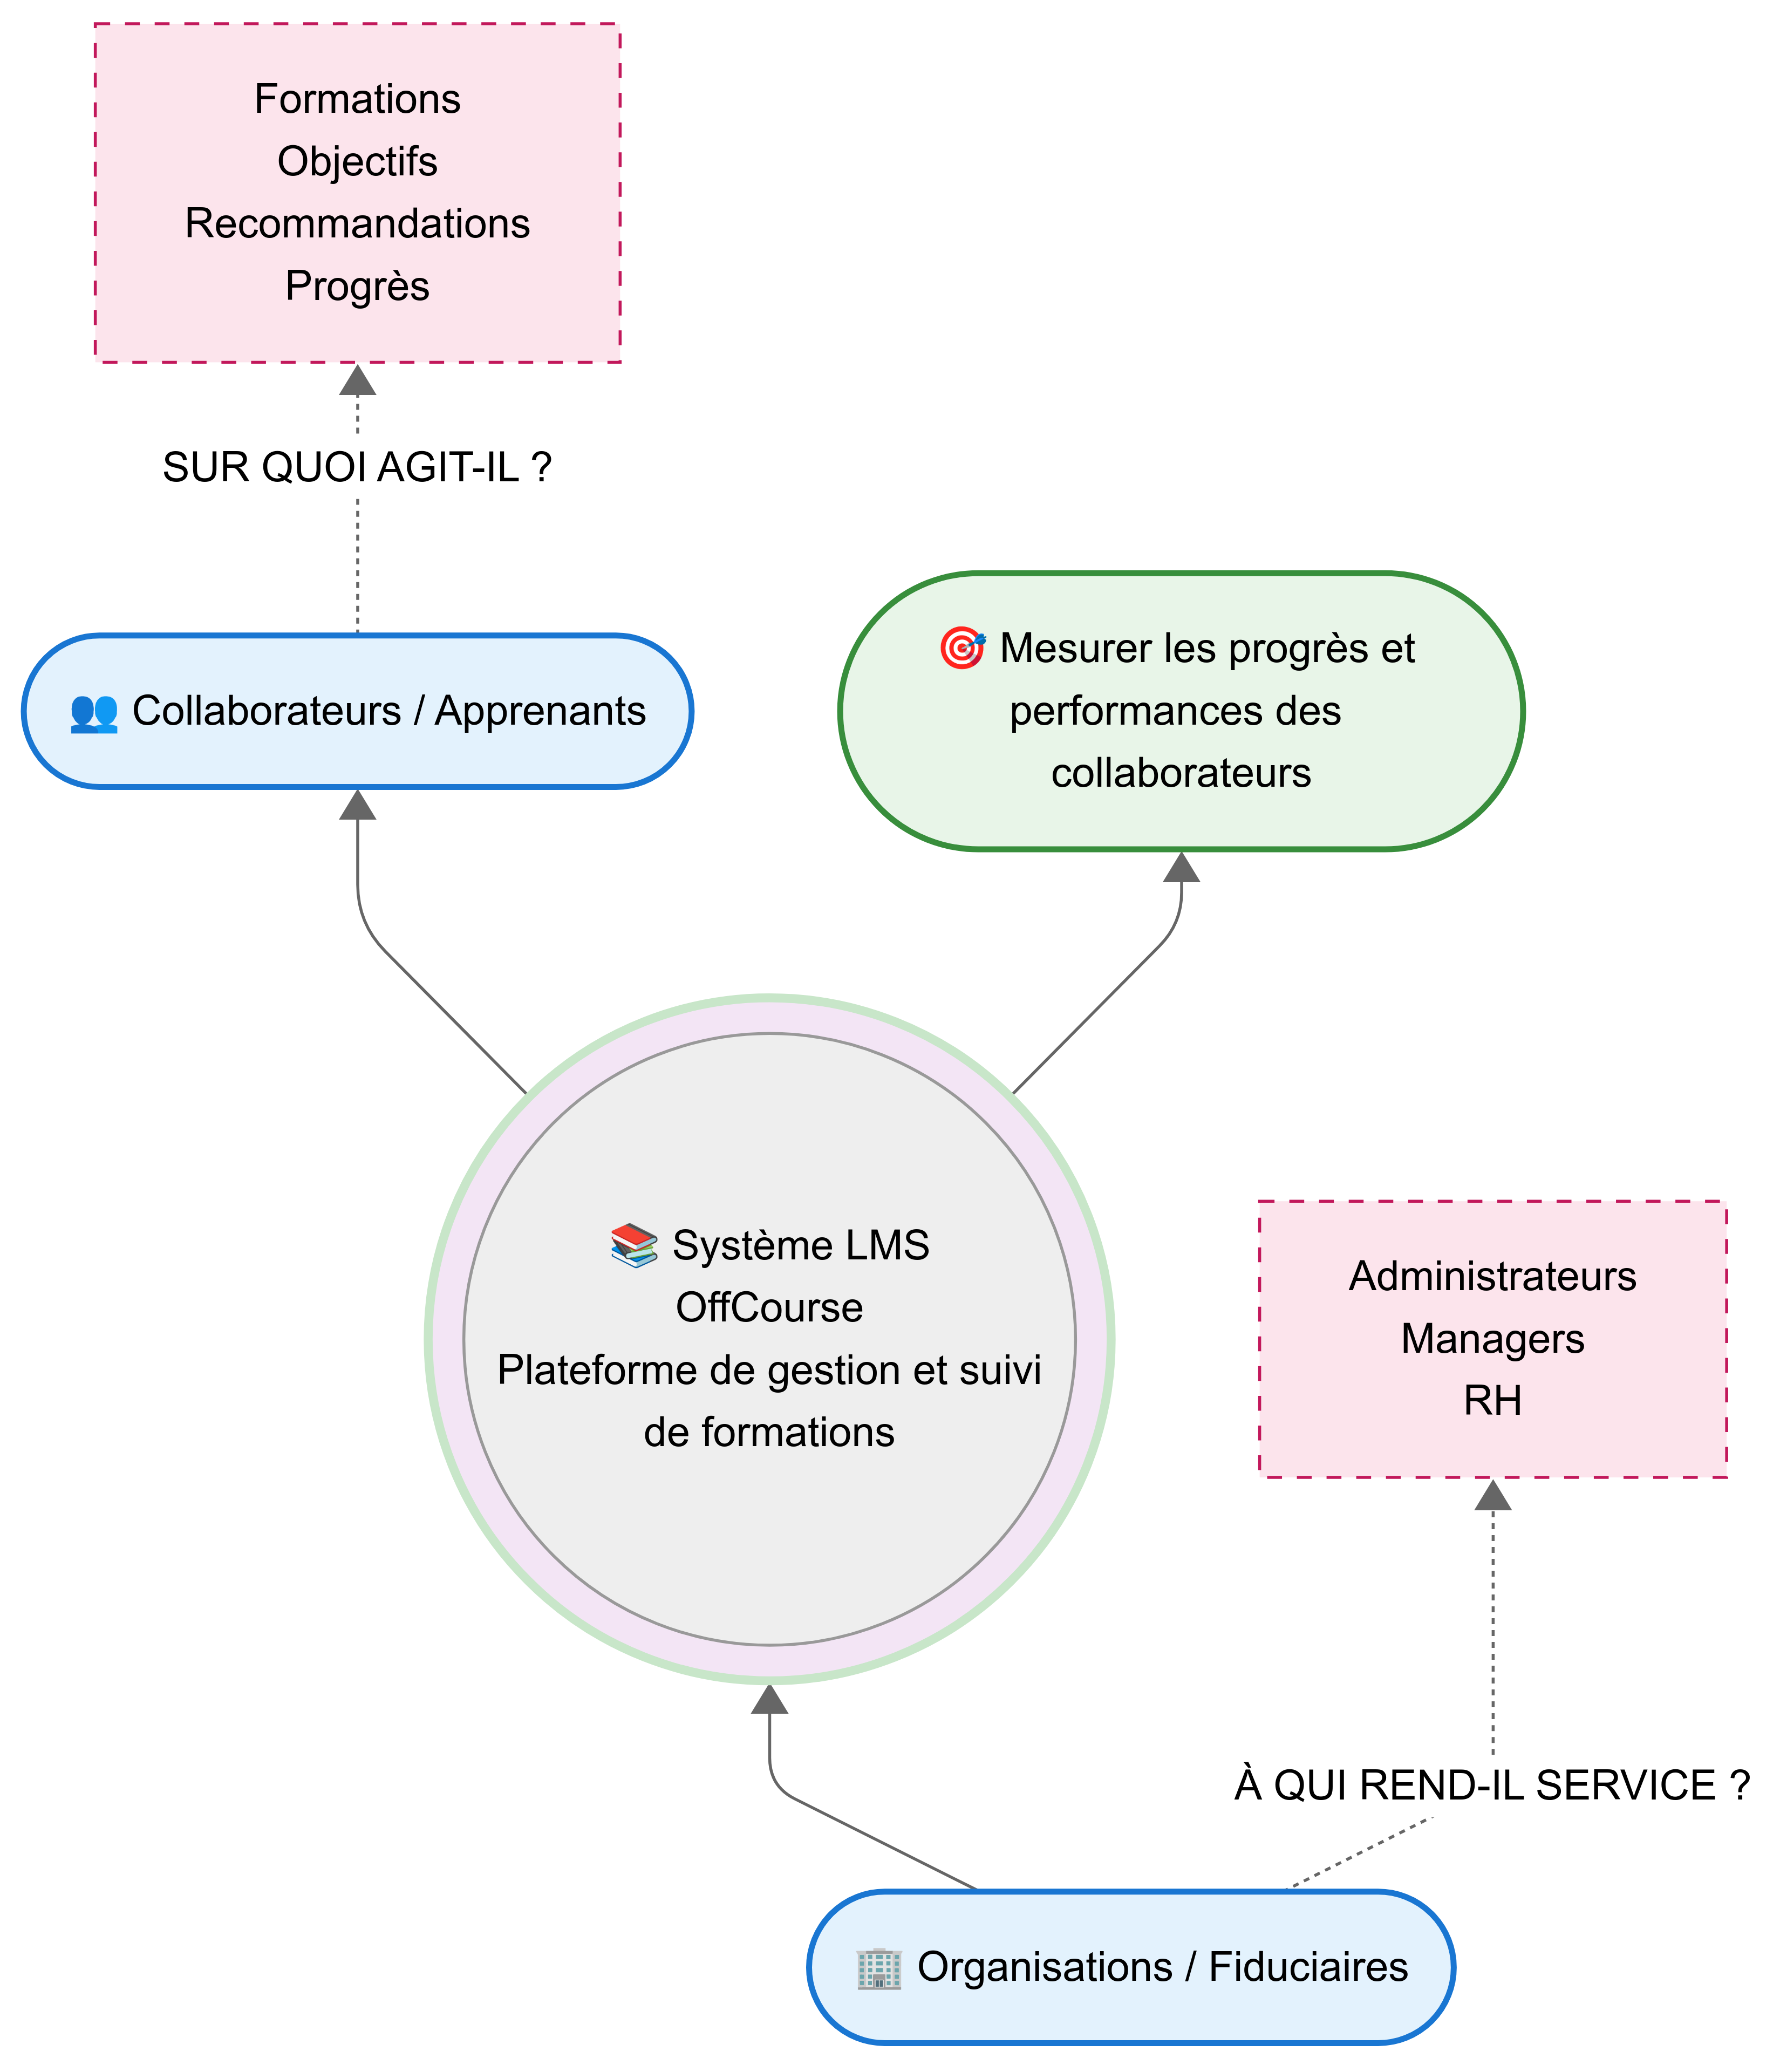
\includegraphics[width=0.85\linewidth]{beteAcorne.png}
\caption{Diagramme Bête à Cornes - System LMS OffCourse}
\end{figure}
\hfill

\vspace{10cm}
\textbf{Analyse du diagramme :}
\begin{itemize}
    \item \textbf{À qui rend-il service ?} Organisations/Fiduciaires, Collaborateurs/Apprenants, Administrateurs/Managers/RH
    \item \textbf{Sur quoi agit-il ?} Formations, Objectifs, Recommandations, Progrès (gestion des trimestres, suivi des objectifs, recommandations de formations)
    \item \textbf{Dans quel but ?} Optimiser la gestion des formations et le développement des compétences au sein des organisations
\end{itemize}

\subsection{Diagrammes de cas d'utilisation}

Les diagrammes de cas d'utilisation permettent de représenter les fonctionnalités du système du point de vue des utilisateurs. Ils offrent un premier pas pour comprendre les
interactions entre le système et ses différents acteurs. En effet, ceux-ci permettent de délimiter le
système en un ensemble de besoins des utilisateurs.
\subsubsection{Cas d'utilisation - Application OffCourse}

Ce diagramme de cas d'utilisation modélise les interactions entre les différents types d'utilisateurs et le système de gestion des formations OffCourse. Il illustre la hiérarchie des acteurs et met en évidence les relations UML essentielles (héritage, inclusion, extension) qui structurent le système.

\begin{figure}[ht!]
\centering
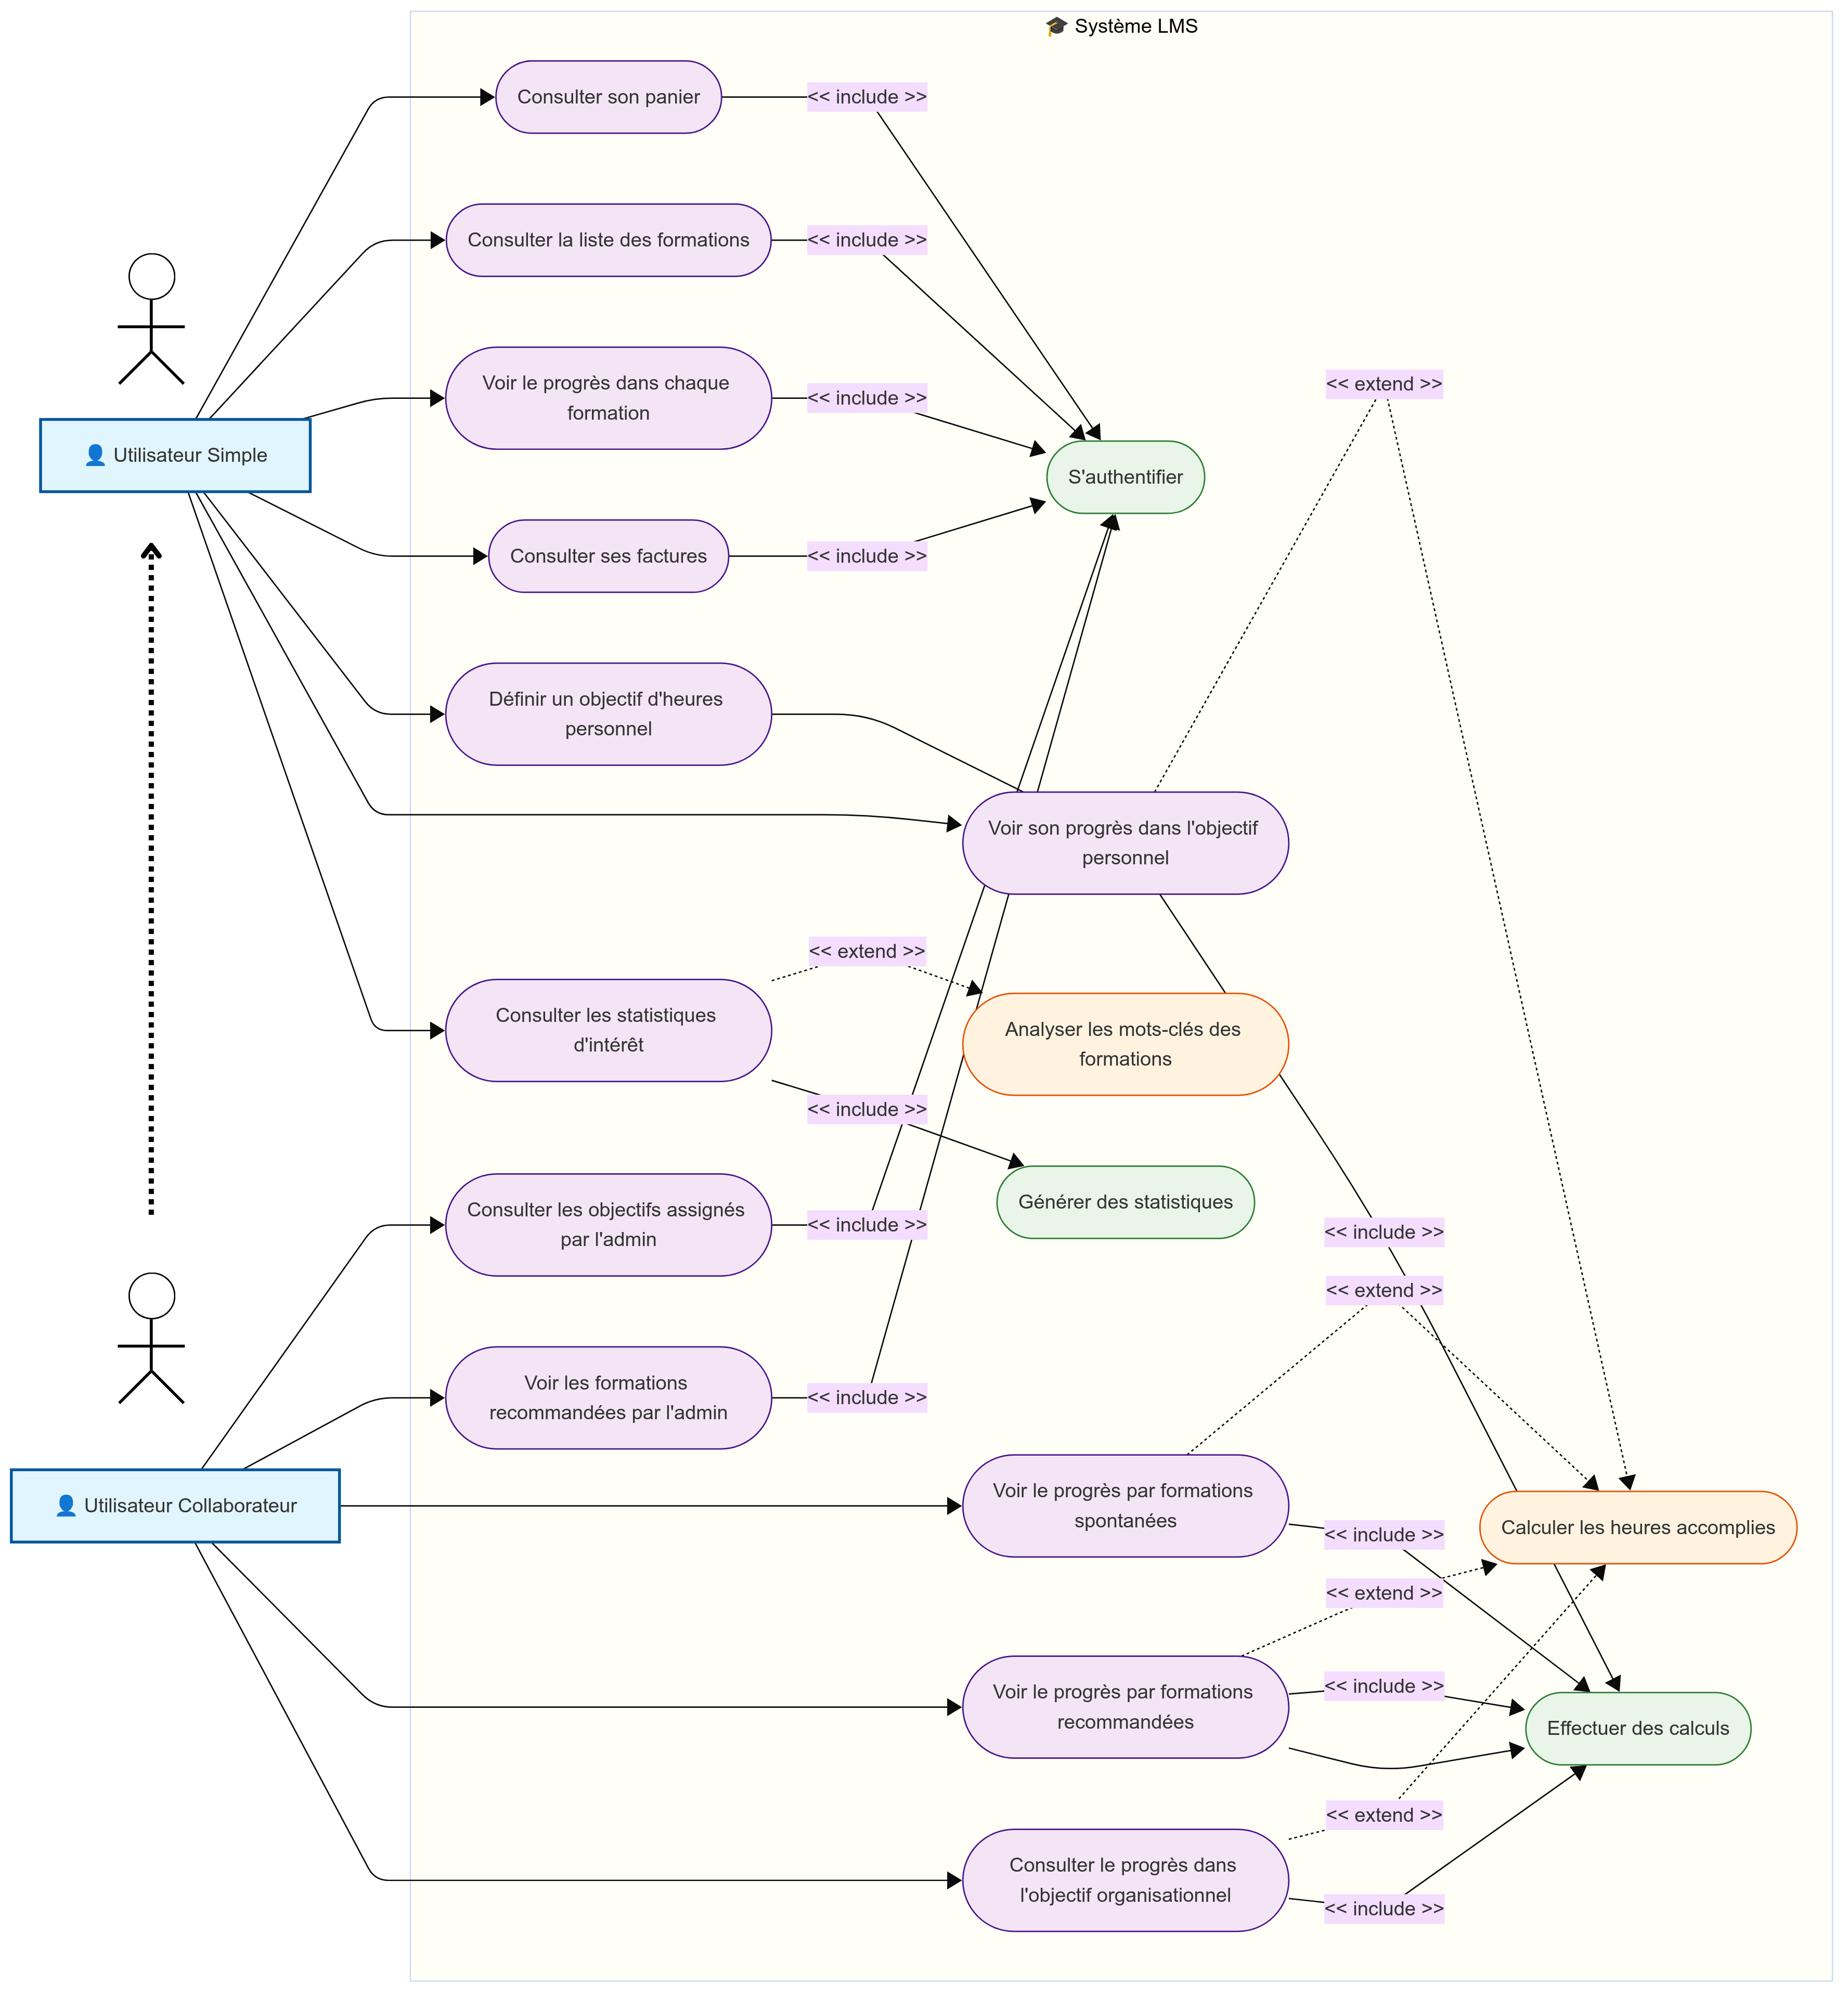
\includegraphics[width=0.85\linewidth]{useCaseoFFcourse.png}
\caption{Diagramme de cas d'utilisation - Gestion des formations OffCourse}
\end{figure}

\textbf{Architecture du système :}

Le diagramme présente une architecture hiérarchique où l'Utilisateur Collaborateur hérite de toutes les fonctionnalités de l'Utilisateur Simple, illustrant ainsi le principe de spécialisation progressive des rôles.

\textbf{Fonctionnalités par acteur :}

\textit{Utilisateur Simple :}
\begin{itemize}
    \item \textbf{Gestion des formations :} Consulter le catalogue des formations disponibles et suivre sa progression dans chaque formation
    \item \textbf{Gestion commerciale :} Consulter son panier d'achat et accéder à l'historique de ses factures
    \item \textbf{Objectifs personnels :} Définir des objectifs d'heures de formation personnalisés et suivre leur réalisation
    \item \textbf{Analyse statistique :} Consulter ses statistiques d'intérêt avec possibilité d'analyse des mots-clés des formations (relation d'extension)
\end{itemize}

\textit{Utilisateur Collaborateur} (hérite de toutes les fonctionnalités de l'Utilisateur Simple) :
\begin{itemize}
    \item \textbf{Gestion organisationnelle :} Consulter les objectifs assignés par l'administrateur de son organisation
    \item \textbf{Formations recommandées :} Accéder aux formations spécifiquement recommandées par l'administration
    \item \textbf{Suivi dual :} Suivre simultanément son progrès dans l'objectif organisationnel et ses formations spontanées
    \item \textbf{Reporting avancé :} Visualiser distinctement le progrès par formations recommandées et formations choisies spontanément
\end{itemize}

\textbf{Relations UML implémentées :}

\begin{itemize}
    \item \textbf{Héritage :} L'Utilisateur Collaborateur hérite des capacités de l'Utilisateur Simple
    \item \textbf{Inclusion (<<include>>) :} Tous les cas d'utilisation incluent l'authentification, les calculs de progression incluent des fonctions de calcul automatique
    \item \textbf{Extension (<<extend>>) :} L'analyse des mots-clés étend optionnellement la consultation des statistiques
    \item \textbf{Associations :} Relations directes entre la définition d'objectifs et leur suivi
\end{itemize}

Cette modélisation garantit une séparation claire des responsabilités tout en permettant une évolutivité du système vers des rôles plus spécialisés.
\hfill
\subsubsection{Cas d'utilisation - Interface LMS United Associate}

Ce diagramme de cas d'utilisation présente l'architecture fonctionnelle complète du système LMS (Learning Management System) de l'application United Associate. Il illustre les interactions entre les différents acteurs et les fonctionnalités disponibles selon leurs rôles et permissions.

\begin{figure}[htbp]
\hspace{2cm}
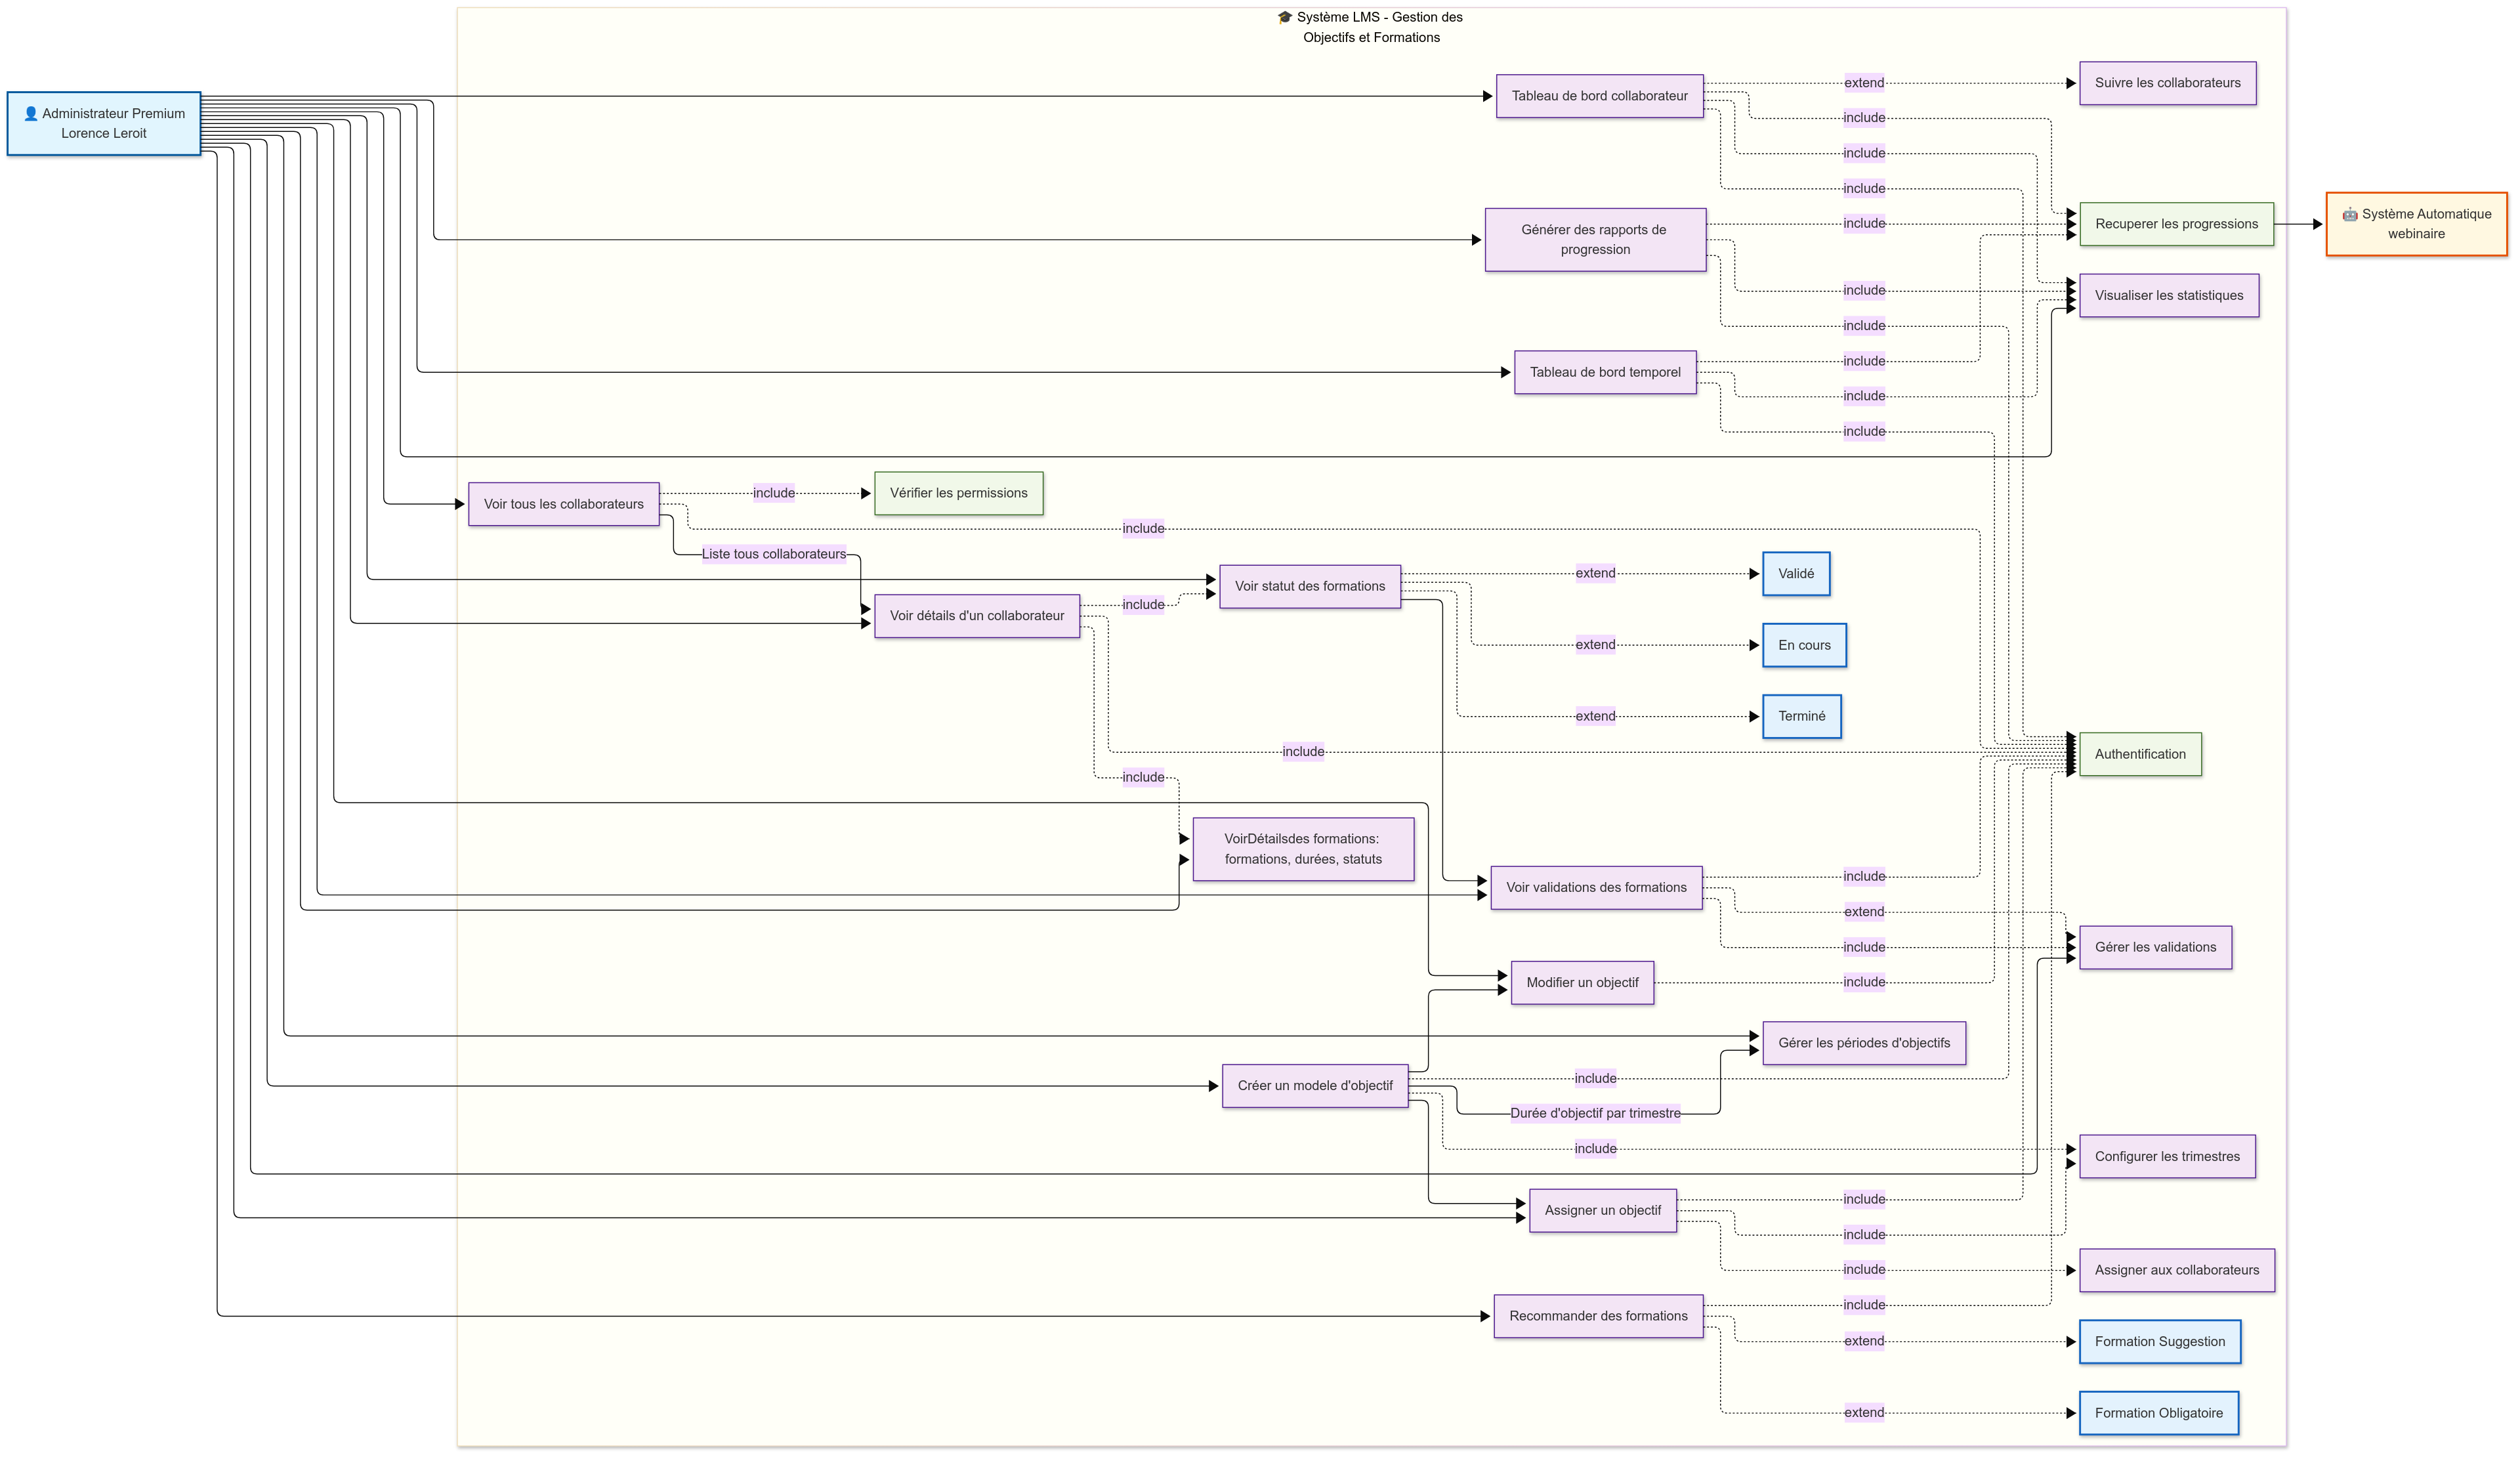
\includegraphics[width=1.25\linewidth, right]{useCaseLMS.png}
\caption{Diagramme de cas d'utilisation - Interface LMS United Associate}
\end{figure}

\paragraph{Acteurs du système :}
\begin{itemize}
    \item \textbf{Collaborateurs} : Utilisateurs finaux qui consultent leurs objectifs, suivent leurs formations et accèdent à leur tableau de bord personnel
    \item \textbf{Système Automatique} : Gère les calculs de progression, les notifications et les mises à jour automatiques
\end{itemize}

\paragraph{Fonctionnalités principales :}

\textbf{Gestion des objectifs et périodes :}
\begin{itemize}
    \item Configuration des trimestres et périodes d'objectifs 
    \item Création et modification d'objectifs avec durées personnalisables 
    \item Assignation d'objectifs spécifiques aux collaborateurs
    \item Suivi des progressions avec calculs automatiques
\end{itemize}

\textbf{Système de formation et recommandations :}
\begin{itemize}
    \item Recommandation de formations avec deux types : \textit{Obligatoire} et \textit{Suggestion}
    \item Assignation de formations spécialisées (taxation, risk management, etc.)
    \item Suivi des statuts de formation : \textit{Terminé}, \textit{En cours}, \textit{Validé}
    \item Système de validation administrateur pour les formations complétées
\end{itemize}

\textbf{Interfaces de suivi et tableaux de bord :}
\begin{itemize}
    \item \textbf{Vue Collaborateur} : Tableau de bord personnel avec indicateurs de progression 
    \item \textbf{Vue Administrateur} : interface de gestion globale avec vue détaillée de tous les collaborateurs.
    \item Historique complet des formations par collaborateur
    \item Génération de rapports et statistiques de performance.
\end{itemize}

\textbf{Fonctionnalités administratives avancées :}
\begin{itemize}
    \item Consultation détaillée des profils collaborateurs
    \item Gestion des validations et approbations de formations.
    \item Suivi global avec compteurs 
    \item Système d'authentification et de gestion des permissions
\end{itemize}

Ce système permet une gestion complète et hiérarchisée des compétences et des formations au sein de l'organisation, avec des outils de suivi adaptés à chaque type d'utilisateur.
\subsection{Diagrammes de séquence du système}

Dans le cadre de la conception du système LMS, les diagrammes de séquence jouent un rôle essentiel en décrivant avec précision l’enchaînement temporel des messages échangés entre les acteurs externes et les différents modules internes. Ils constituent un support précieux pour comprendre, valider et communiquer la logique de fonctionnement du système tout au long de son cycle de vie.

\subsubsection{Séquence — Utilisateur OffCourse}

Le diagramme de séquence ci-après met en lumière l’ensemble des interactions qu’un utilisateur peut avoir avec la plateforme OffCourse. Il permet de visualiser, étape par étape, la manière dont les demandes de l’utilisateur sont traitées par le système et comment les modules collaborent pour assurer une expérience fluide et cohérente:


% Première partie du diagramme
\begin{figure}[ht!]
\hspace{2cm}
    \adjustbox{trim=0 {.48\height} 0 0, clip, width=1.2\linewidth, right}{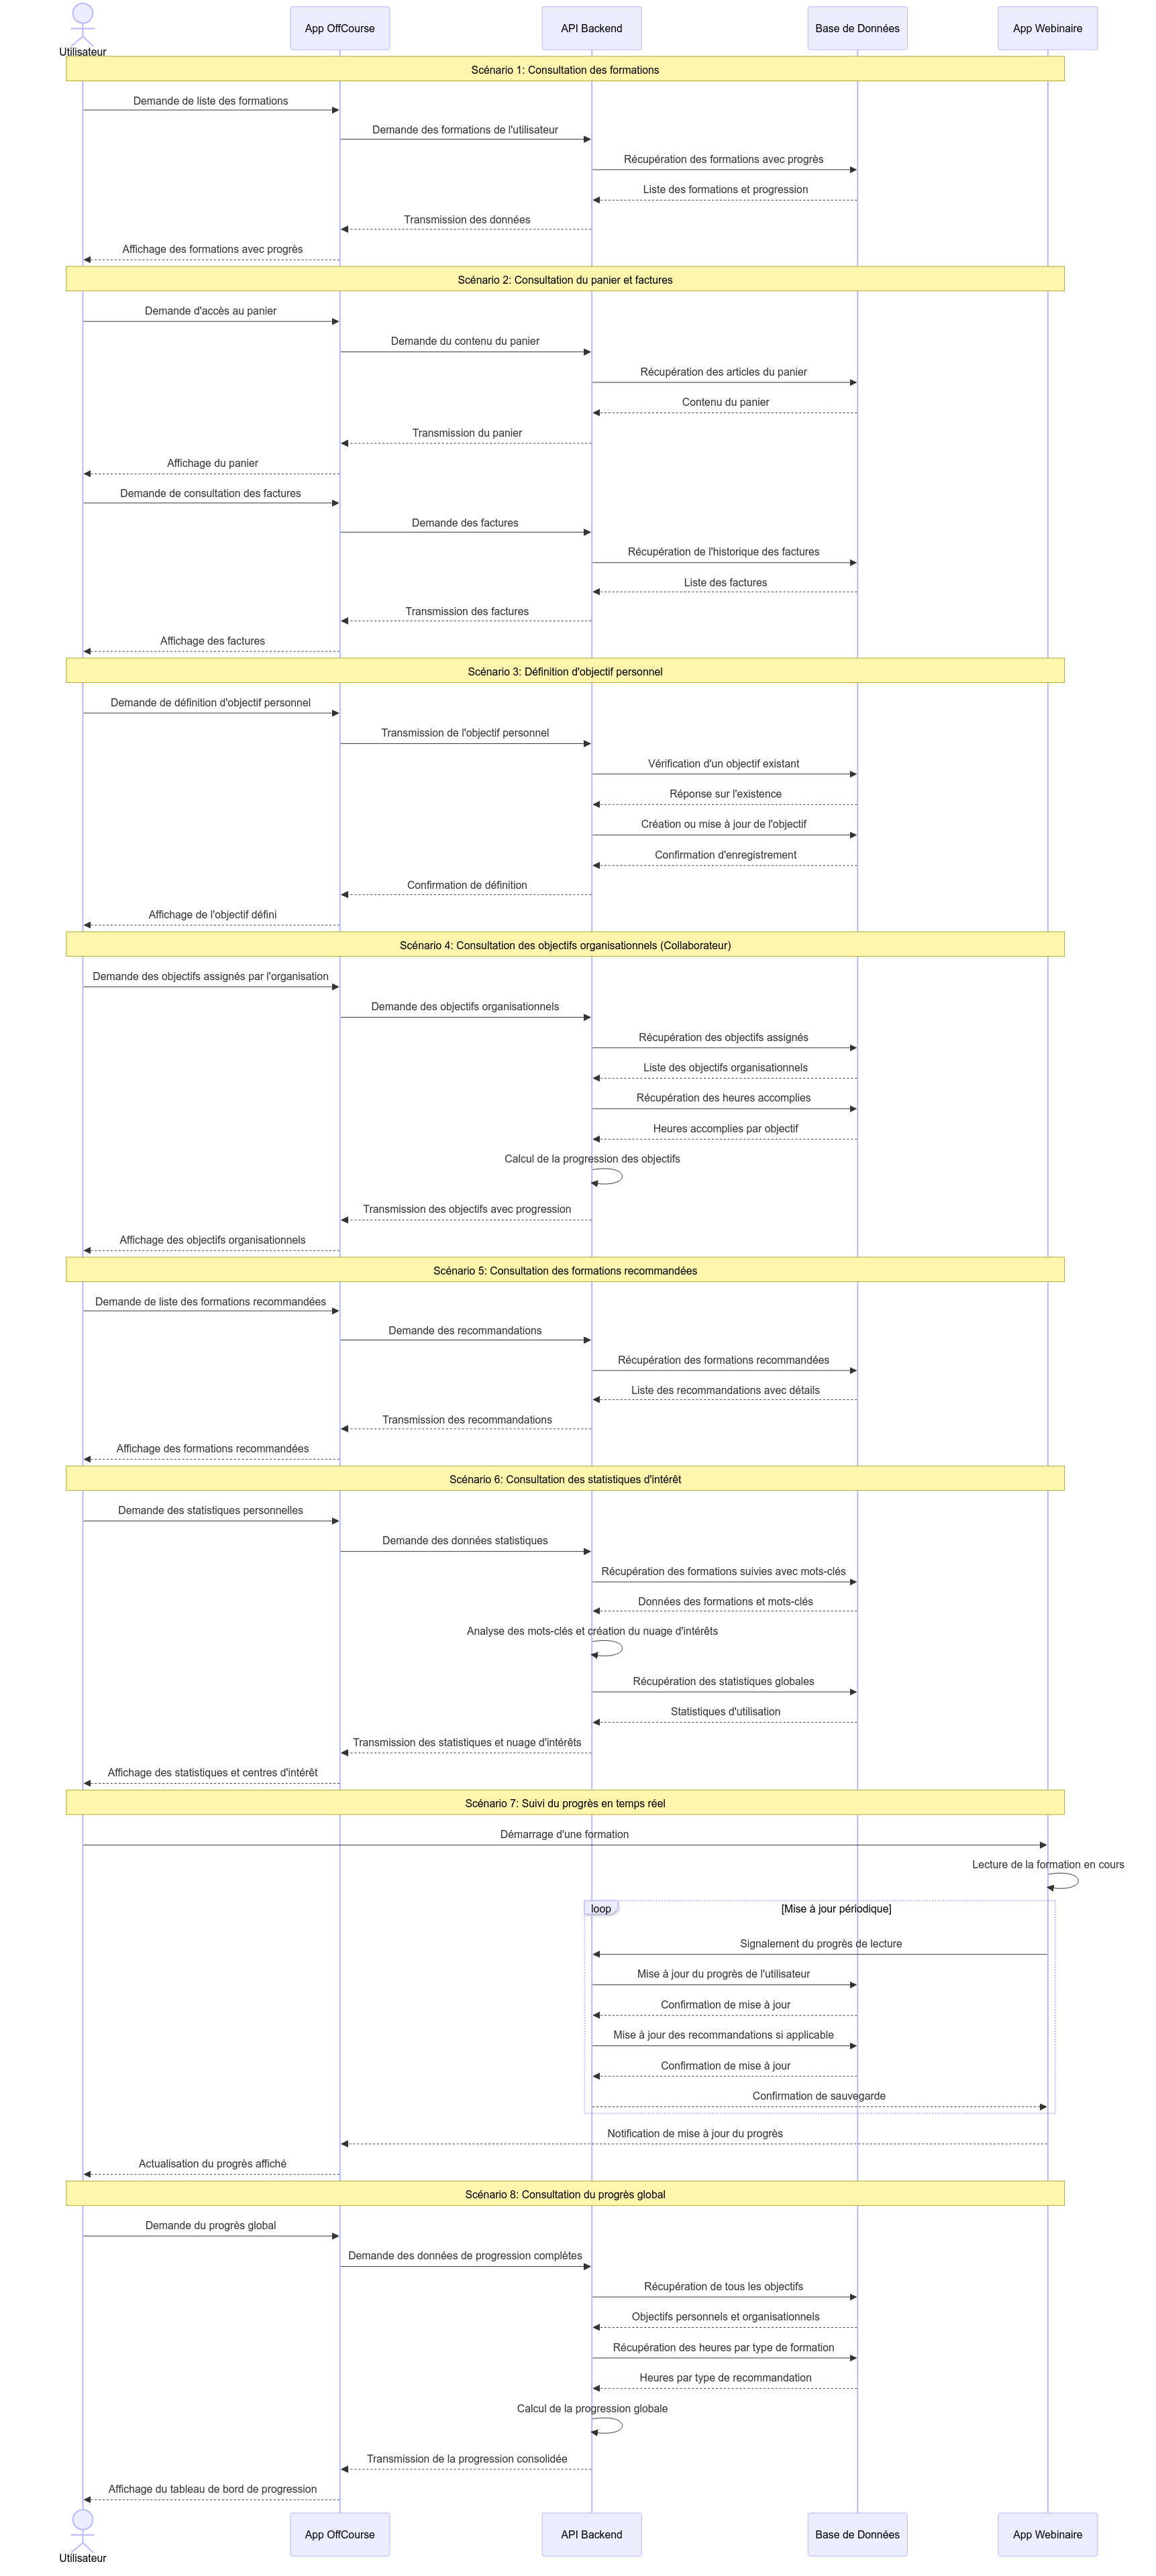
\includegraphics{sequenceLMS.png}}
    \caption{Diagramme de séquence — Interactions utilisateur OffCourse (Partie 1)}
\end{figure}

\newpage

% Deuxième partie du diagramme
\begin{figure}[ht!]
\hspace{2cm}
    \adjustbox{trim=0 0 0 {.49\height}, clip, width=1.2\linewidth, right}{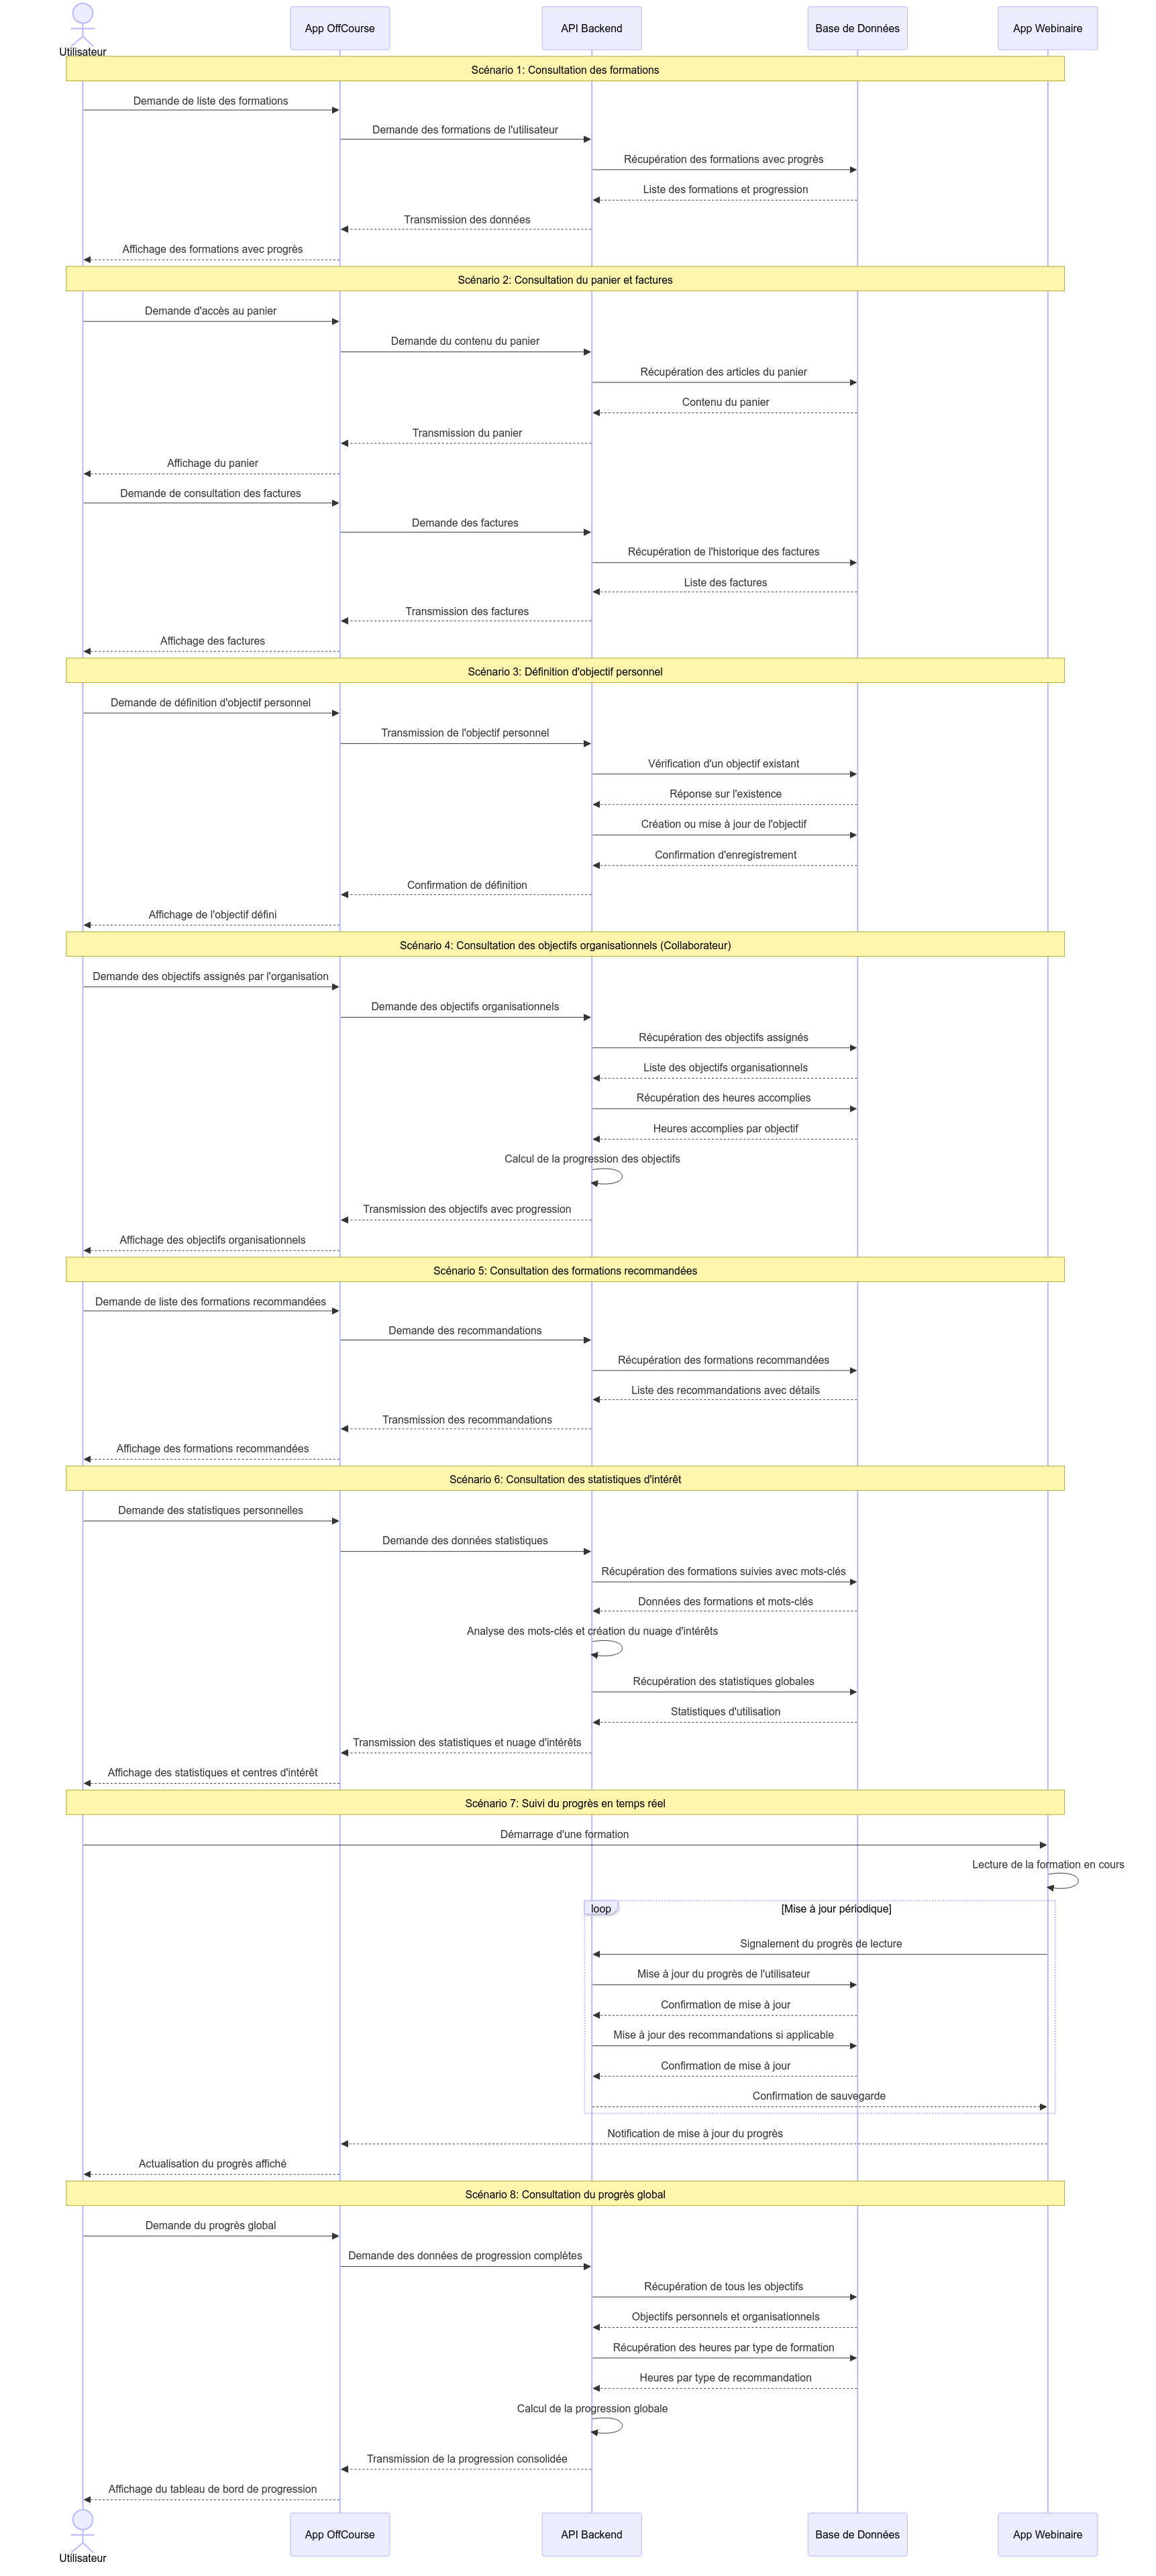
\includegraphics{sequenceLMS.png}}
    \caption{Diagramme de séquence — Interactions utilisateur OffCourse (Partie 2)}
\end{figure}

Dans ces scénarios, l’utilisateur consulte les formations mises à sa disposition, gère ses objectifs de formation à la fois individuels et organisationnels et reçoit des recommandations adaptées à ses besoins spécifiques. Le suivi de la progression est également automatisé grâce à une communication constante entre les composants internes, garantissant ainsi la mise à jour en temps réel des indicateurs de performance. De plus, ce diagramme révèle comment le système orchestre la synchronisation des données pour préserver l’intégrité et la cohérence des informations affichées à l’utilisateur.
L’étude de ce diagramme est primordiale pour vérifier la robustesse des processus de gestion des formations et des recommandations, et pour identifier d’éventuelles optimisations susceptibles d’améliorer l’efficacité globale de la plateforme.

\begin{itemize}
    \item Consultation et sélection de contenus pédagogiques adaptés.
    \item Gestion et paramétrage des objectifs de formation personnels et collectifs.
    \item Visualisation du niveau d’avancement et réception de suggestions personnalisées.
    \item Synchronisation continue entre les modules pour garantir la fiabilité des données.
\end{itemize}


\subsubsection{Séquence — Administrateur United Associate}

Le second diagramme de séquence présente de manière détaillée les principales opérations réalisées par un administrateur au sein de l’environnement LMS de United Associate. Il sert de référence pour analyser les responsabilités de gestion et de supervision confiées aux administrateurs, ainsi que pour vérifier la bonne circulation des informations entre les différents services du système.
\begin{figure}[ht!]
\hspace{1.5cm}
    \adjustbox{trim=0 {.65\height} 0 0 , clip, width=1.2\linewidth, right}
% \begin{figure}[htbp]
% \centering
{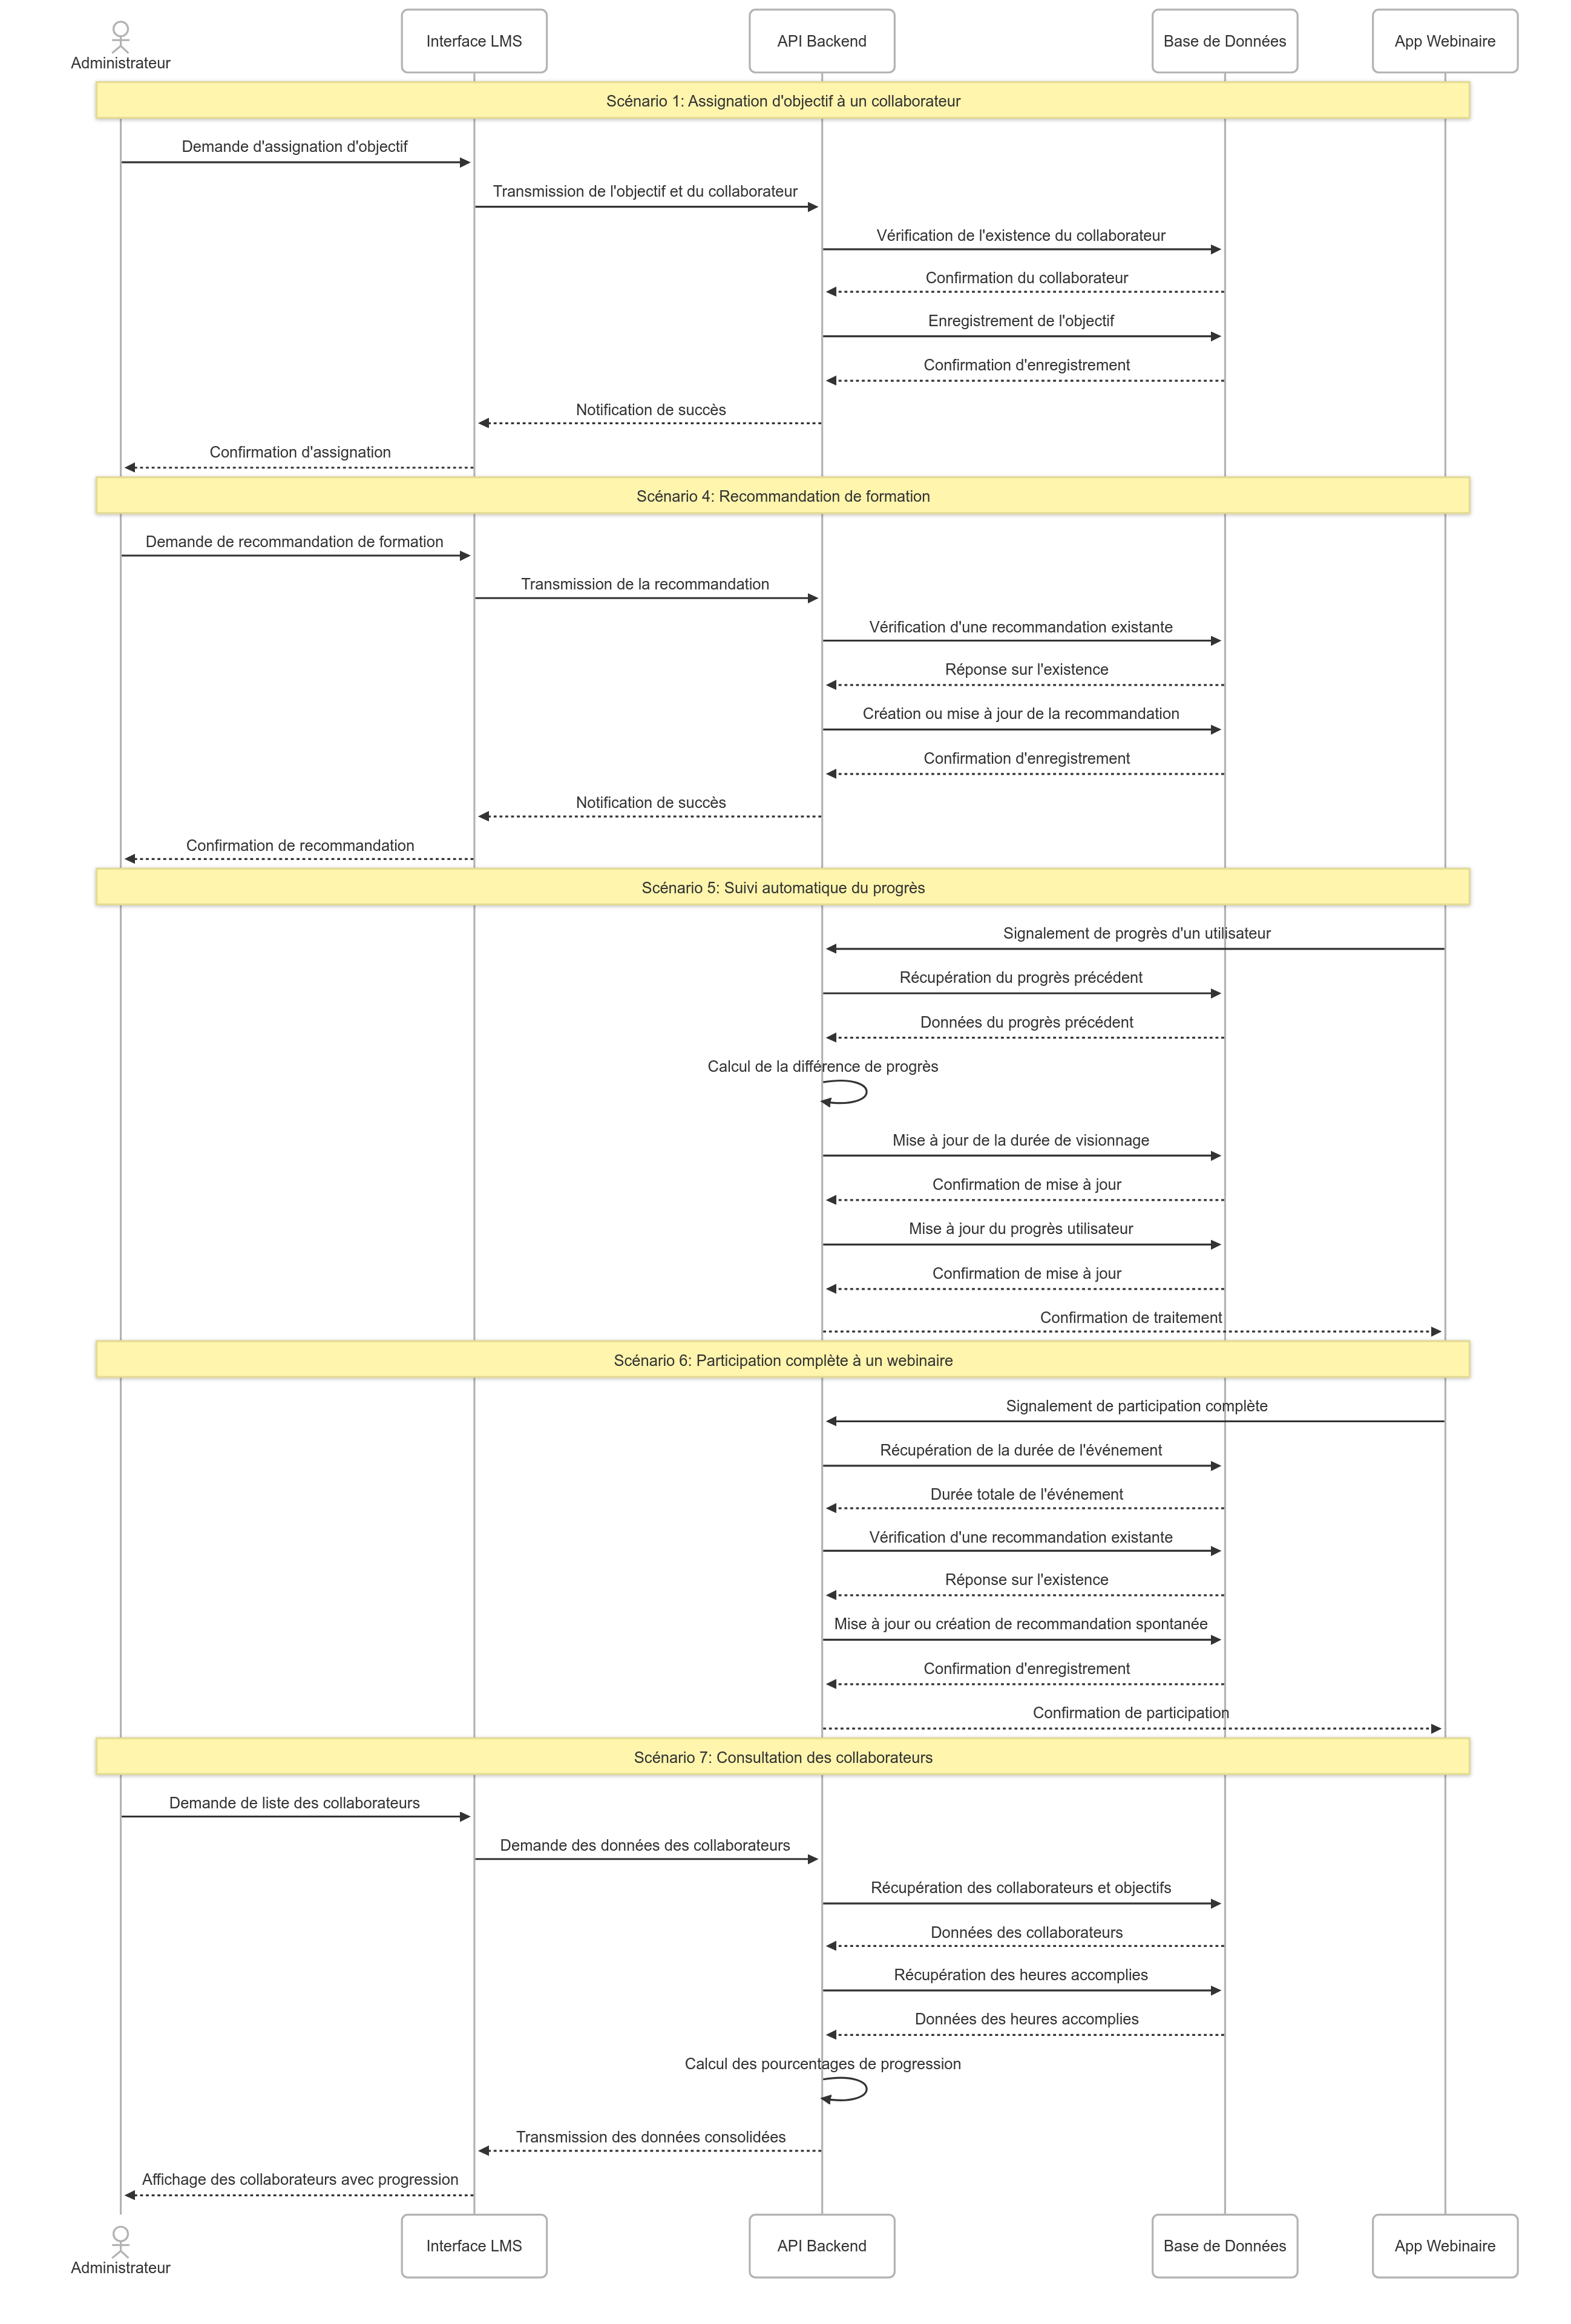
\includegraphics[width=1\linewidth]{sequenceAdmin.png}}
\caption{Diagramme de séquence — Processus administratif LMS United Associate}
\end{figure}
\begin{figure}[ht!]
\hspace{1.5cm}
    \adjustbox{trim=0 0 0 {.25\height} , clip, width=1.2\linewidth, right}
% \begin{figure}[htbp]
% \centering
{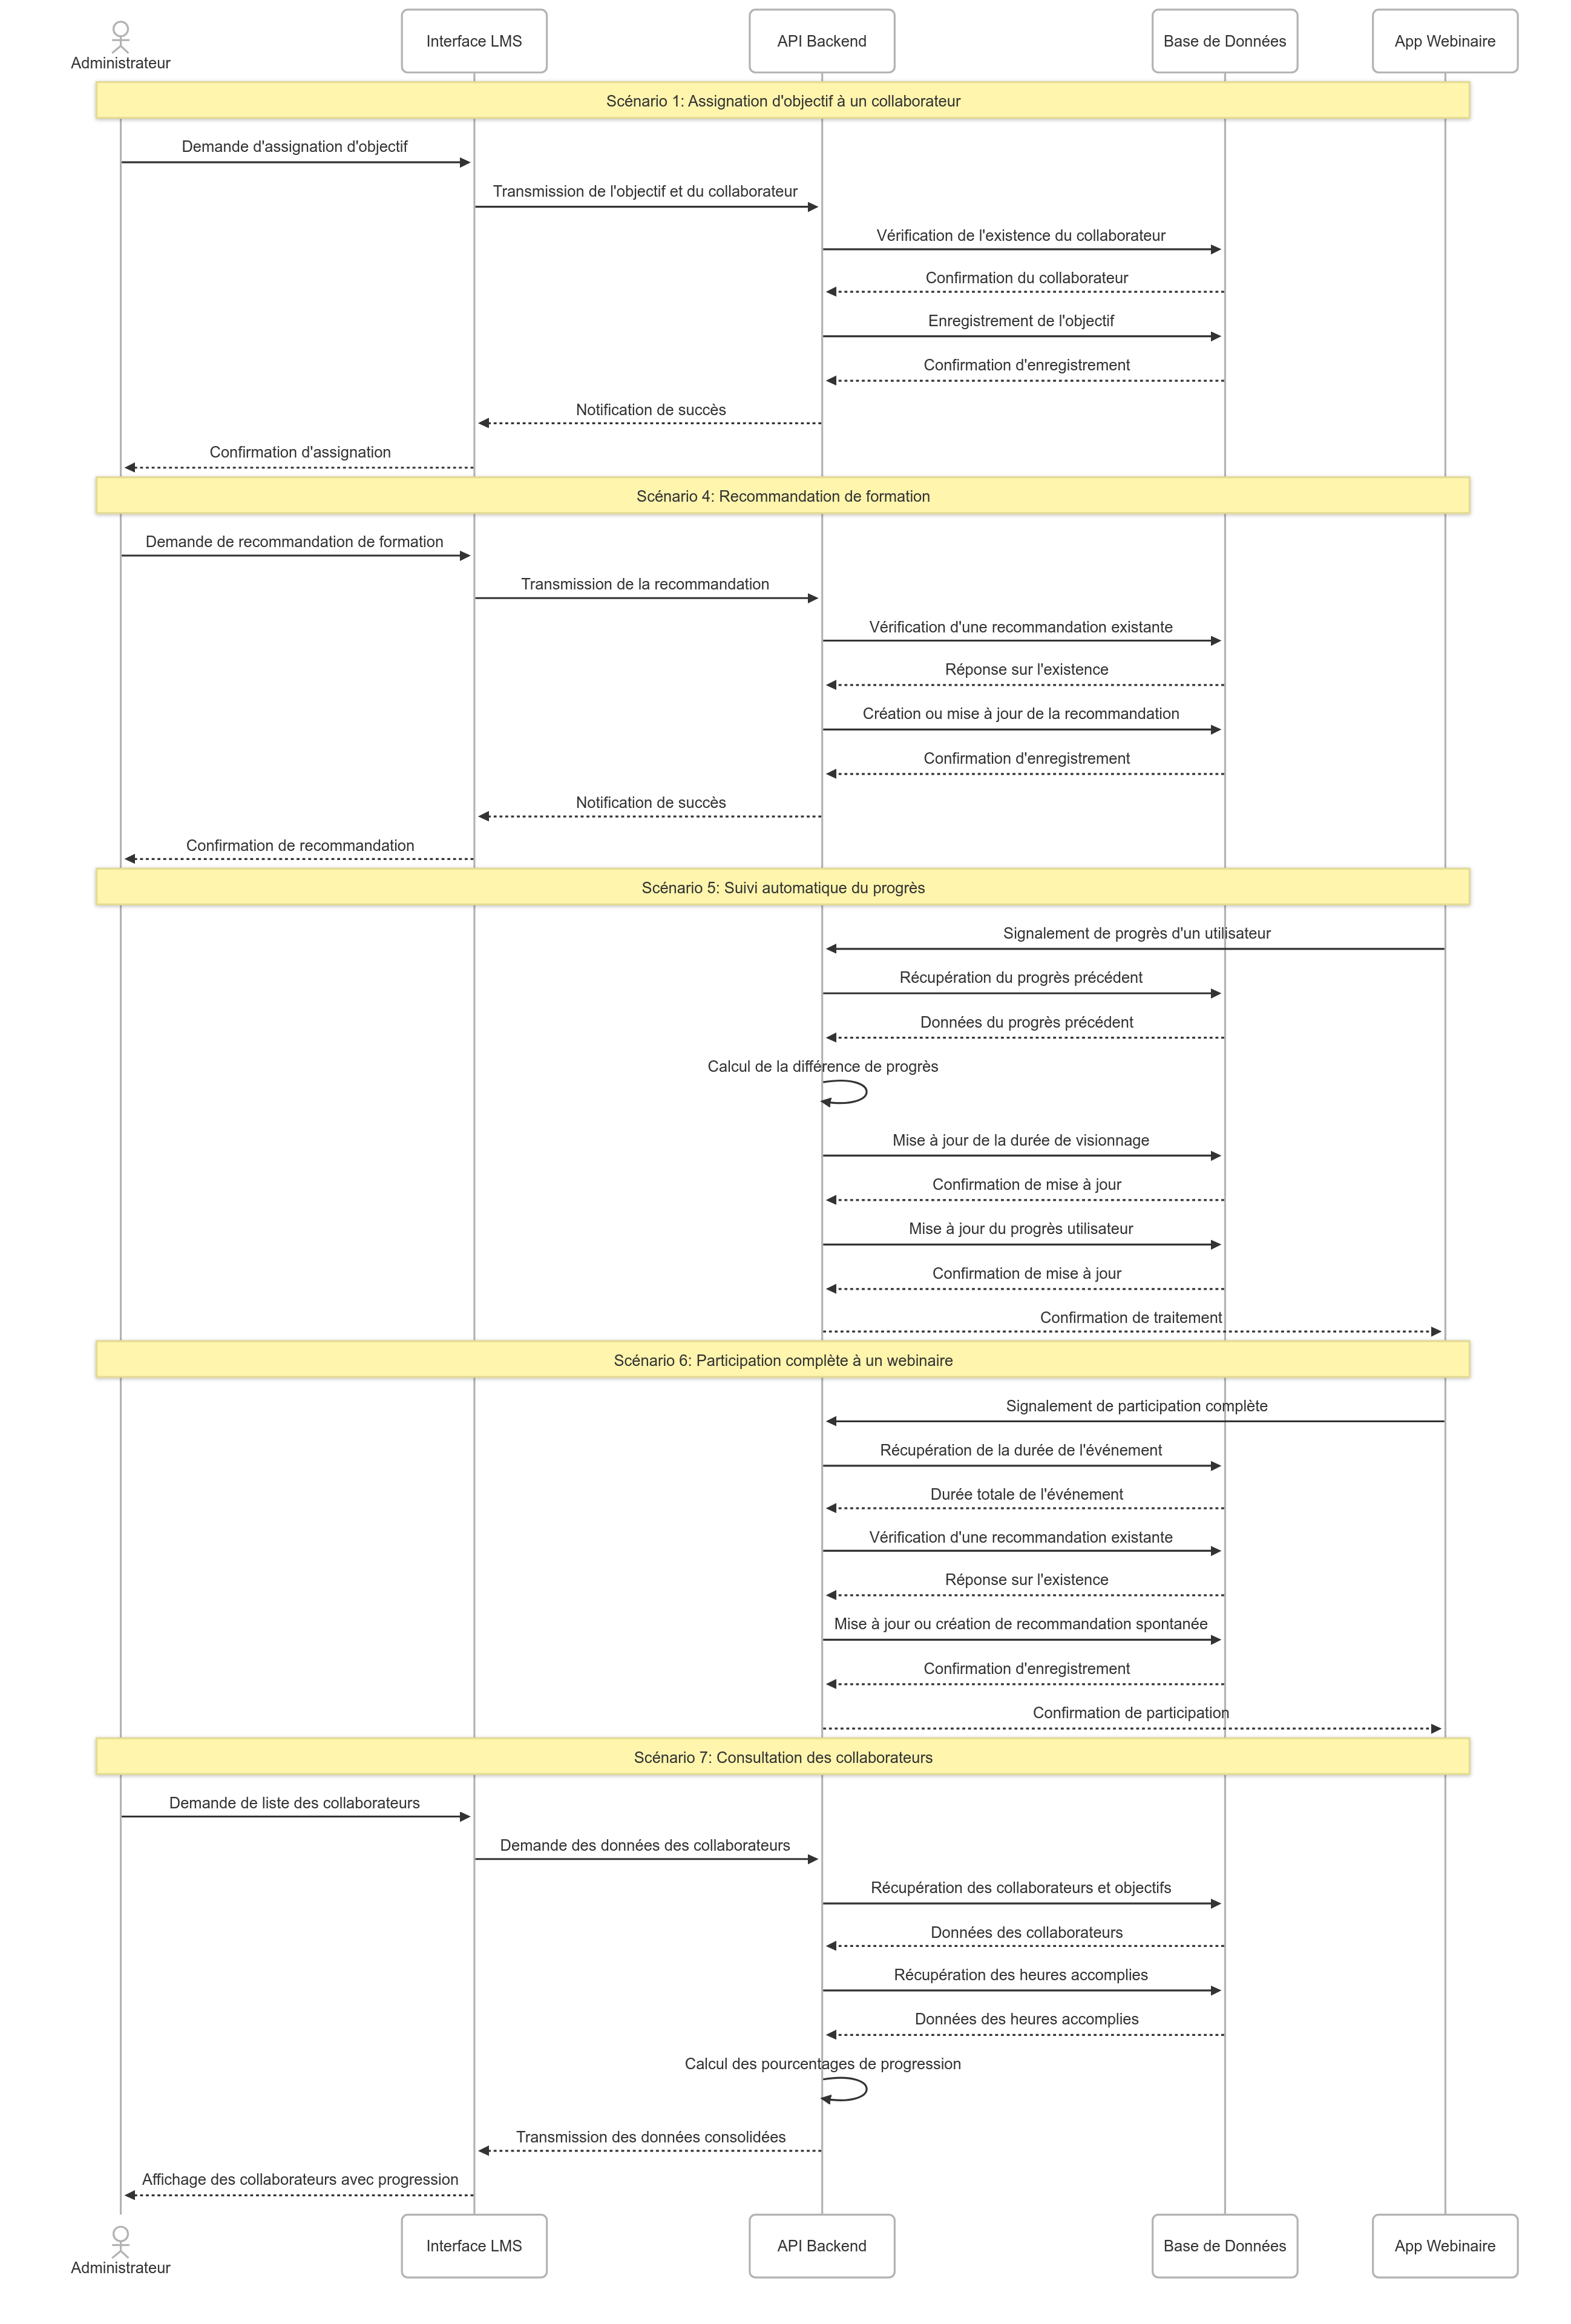
\includegraphics[width=1\linewidth]{sequenceAdmin.png}}
\caption{Diagramme de séquence — Processus administratif LMS United Associate}
\end{figure}
\\
À travers ces scénarios, l’administrateur définit les périodes de formation en créant et configurant les trimestres, puis attribue des objectifs aux collaborateurs selon les besoins pédagogiques identifiés. Il procède ensuite à la recommandation de formations spécifiques, en veillant à ce que celles-ci répondent aux exigences de montée en compétences du personnel. Le système assure en parallèle le suivi automatique de l’avancement, ce qui permet à l’administrateur de consulter des rapports à jour sans intervention manuelle. Cette automatisation réduit considérablement la charge de travail tout en renforçant la précision des données collectées.

Ce diagramme confirme que le rôle de l’administrateur est central pour maintenir l’efficacité et la pertinence du dispositif de formation continue. Il permet également d’anticiper d’éventuelles évolutions futures pour intégrer de nouvelles fonctionnalités administratives.

\begin{itemize}
    \item Définition et paramétrage des périodes trimestrielles de formation.
    \item Attribution d’objectifs spécifiques en fonction du profil des collaborateurs.
    \item Sélection et recommandation de formations ciblées.
    \item Suivi et mise à jour automatisés du niveau d’accomplissement des objectifs.
    \item Consultation et analyse des données individuelles et collectives des collaborateurs.
\end{itemize}


\subsection{Modèle du domaine}

Le modèle du domaine représente les concepts métier et leurs relations dans le contexte du système LMS.

\begin{figure}[ht!]
\hspace{2cm}
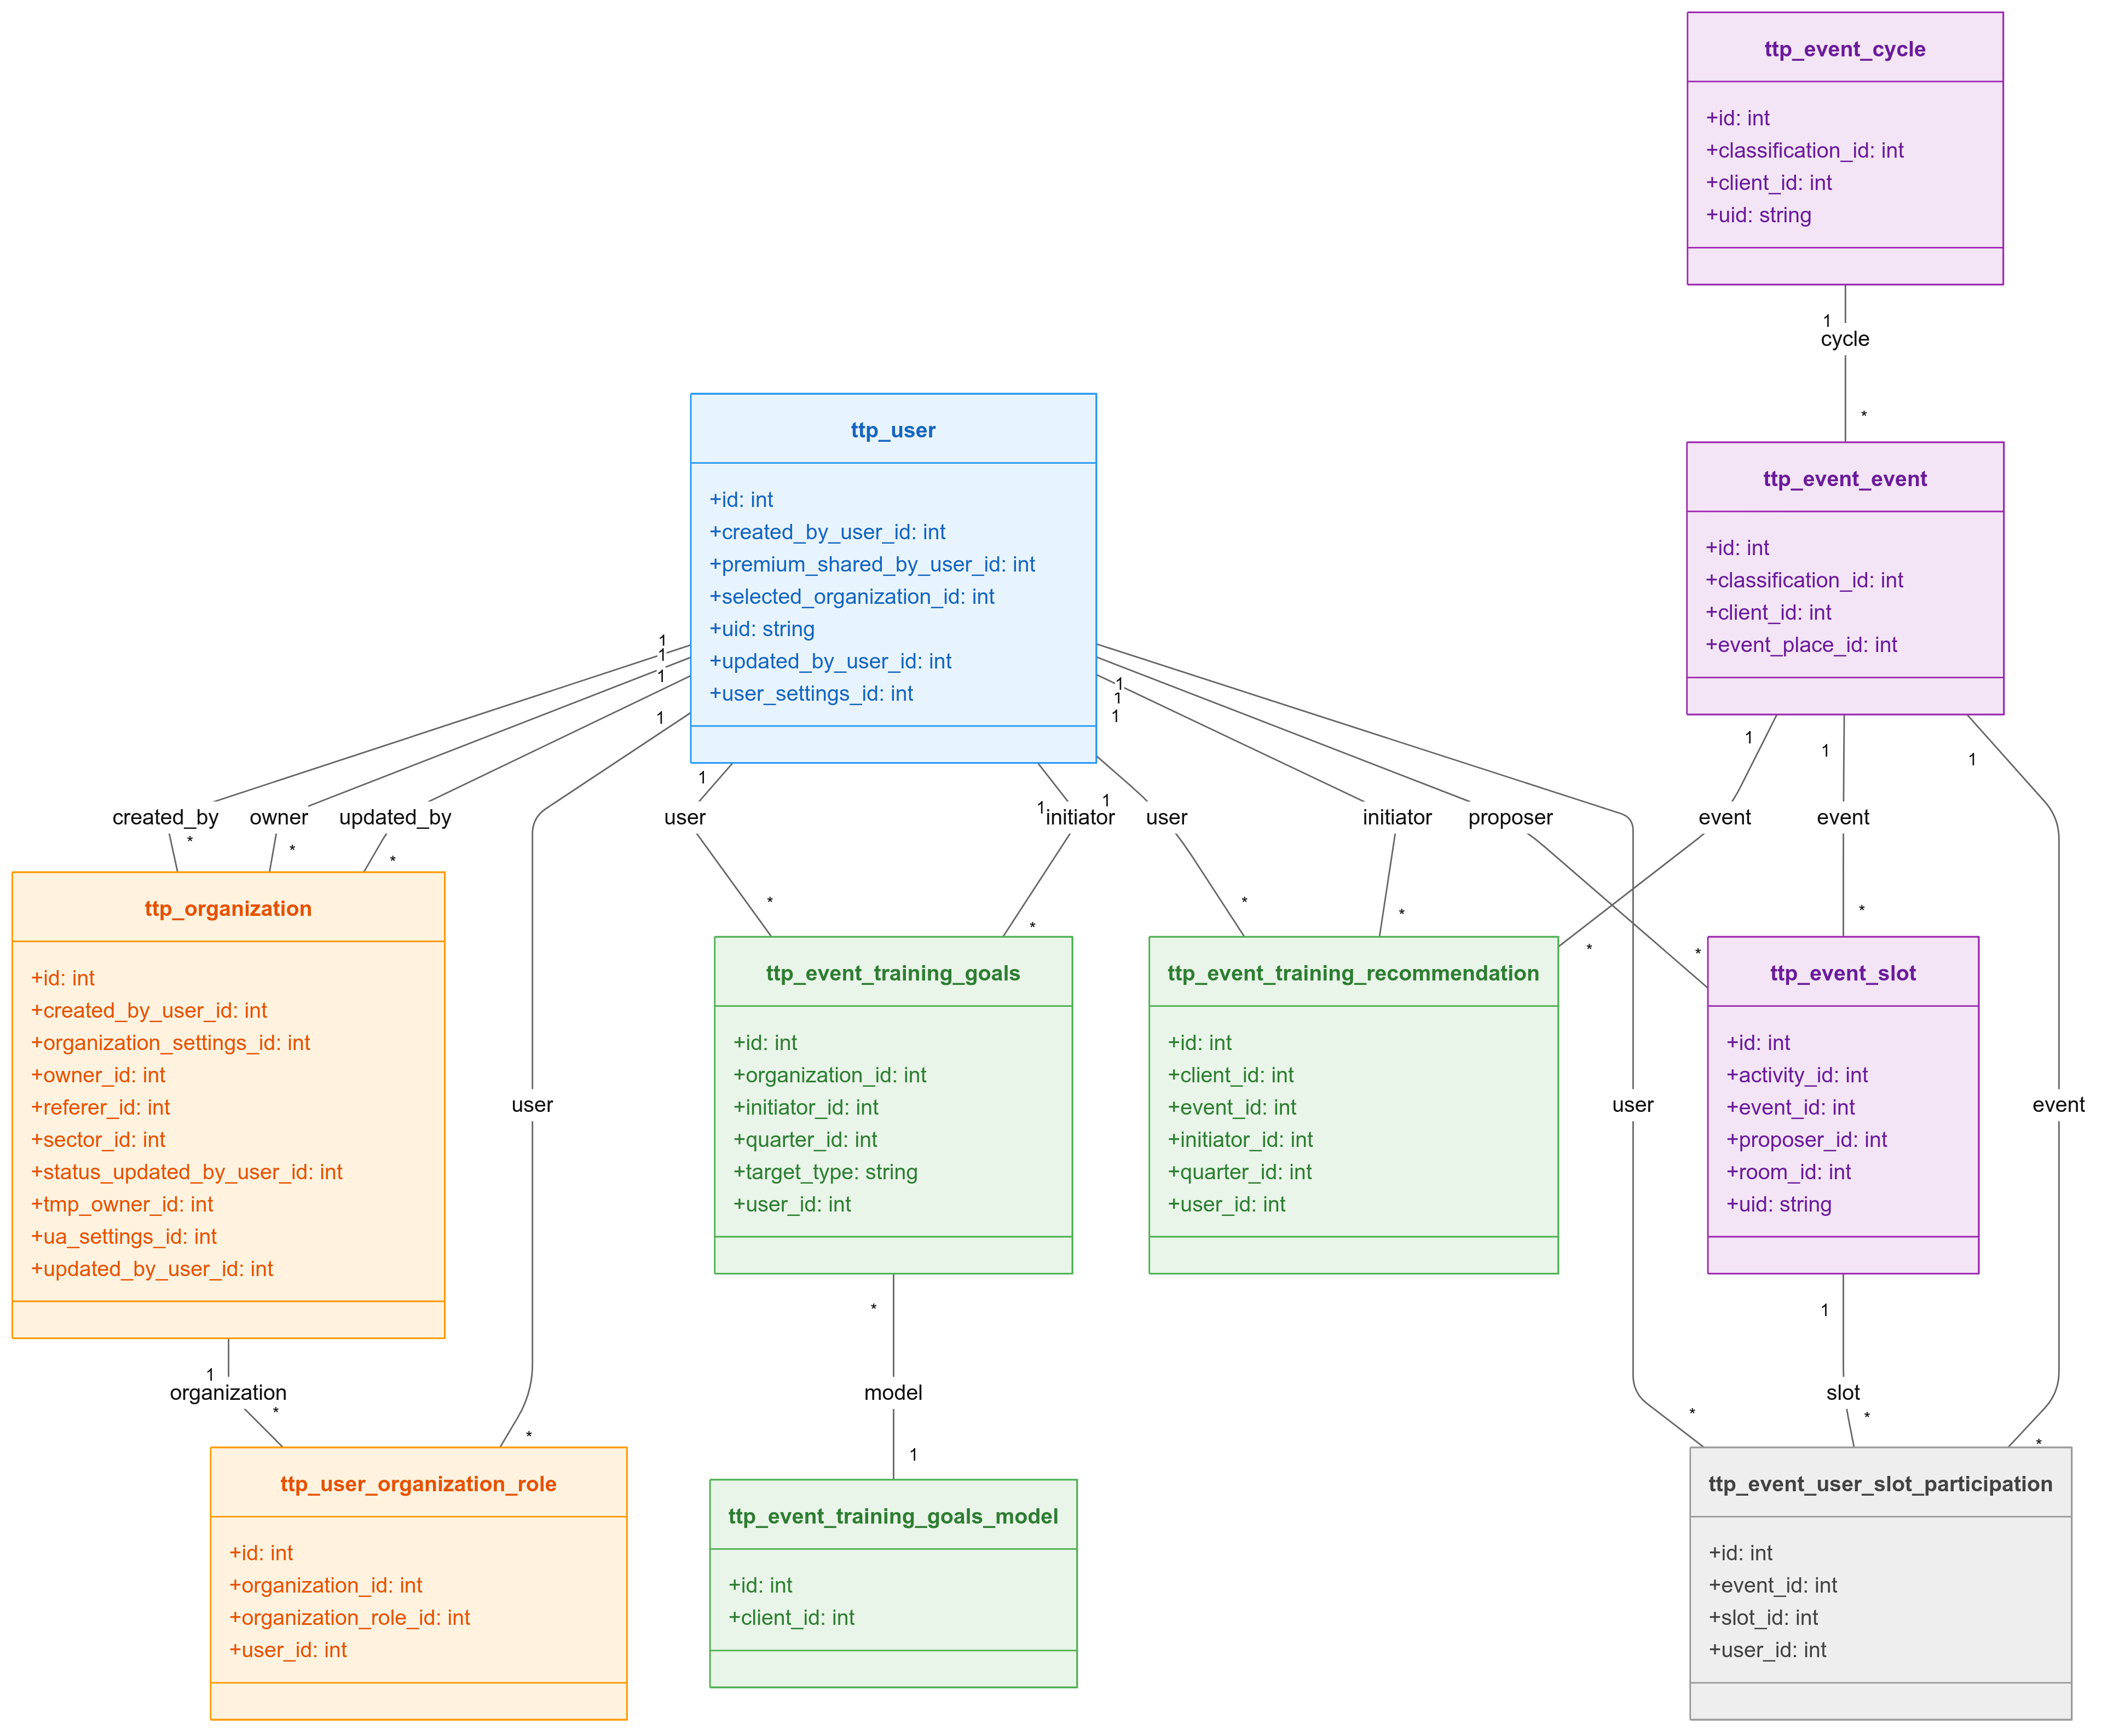
\includegraphics[width=1.2\linewidth,right]{Editor _ Mermaid Chart-2025-06-10-161411.png}
\caption{Modèle du domaine - Système LMS}
\end{figure}
\textbf{Analyse du modèle :}

Le modèle révèle une architecture centrée sur l'entité \texttt{User} qui peut jouer différents rôles selon son contexte organisationnel. Les entités principales sont :

\begin{itemize}
    \item \textbf{User} : Entité centrale représentant tous les utilisateurs du système
    \item \textbf{Organization} : Structure regroupant les collaborateurs
    \item \textbf{Role} : Définit les privilèges d'accès (official, admin)
    \item \textbf{Quarter} : Période temporelle pour l'organisation des formations
    \item \textbf{TrainingGoal} : Objectifs de formation avec cibles horaires
    \item \textbf{Recommendation} : Suggestions de formations avec typologie
    \item \textbf{Event} : Formations et événements disponibles
    \item \textbf{UserSlotParticipation} : Suivi de la participation et du progrès
\end{itemize}

Les relations entre ces entités permettent de gérer la complexité des interactions organisationnelles tout en maintenant la flexibilité nécessaire pour les utilisateurs individuels.

\section{Conclusion}

Ce chapitre d'analyse et de conception a permis d'établir une base solide pour le développement du système LMS. L'utilisation d'UML nous a fourni un langage commun pour exprimer les besoins et modéliser l'architecture du système.

Les principaux résultats de cette phase d'analyse sont :

\begin{itemize}
    \item \textbf{Identification claire des acteurs} et de leurs besoins spécifiques
    \item \textbf{Modélisation complète des fonctionnalités} requises pour chaque type d'utilisateur
    \item \textbf{Architecture logique cohérente} supportant les besoins organisationnels et individuels
    \item \textbf{Spécifications détaillées} des interactions système-utilisateur
    \item \textbf{Modèle de données} robuste pour supporter l'évolutivité du système
\end{itemize}

Cette analyse constitue le fondement technique sur lequel s'appuiera la phase de développement. Elle garantit que le système répondra aux attentes des utilisateurs tout en respectant les contraintes de performance, sécurité et maintenabilité identifiées.

Le chapitre suivant présentera les choix technologiques et l'architecture technique détaillée du système, en s'appuyant sur les spécifications définies dans cette phase d'analyse.